\documentclass[a4paper,12pt]{article}
\usepackage[utf8]{inputenc}
\usepackage[T1]{fontenc}
\usepackage[hungarian]{babel}
\usepackage{graphicx}
\usepackage{geometry}
\geometry{a4paper,
		     tmargin = 35mm, 
		     lmargin = 25mm,
		     rmargin = 30mm,
		     bmargin = 30mm}
\usepackage{mathtools}
\usepackage{amsmath}
\usepackage{color}
\usepackage{setspace}
\usepackage{amsmath,amssymb}
\usepackage{float}
\usepackage{hyperref}

\usepackage{indentfirst}
\usepackage{subfig}

\usepackage{siunitx}

\renewcommand\thesection{\Roman{section}}

\begin{document}

\linespread{1.25}

\begin{titlepage}

	\centering
	
\includegraphics[width=0.66\textwidth]{elte.jpg}\par\vspace{1cm}
	{\scshape\LARGE ELTE TTK \par}
	\vspace{3cm}
	{\scshape\Large Dinamikus nano- és mikrokeménység mérése \par}
	\vspace{1cm}
	{\large\itshape Olar Alex\par}
	\vspace{3cm}
	{\large 2018 \par}
	
\end{titlepage}

\tableofcontents

\newpage

\section{Elméleti összefoglaló, mérési eszközök}

\par A mérés során egy keménységmérő eszközt ismertünk meg, amely Vickers-fejjel végezte el a méréseket. Ezek során tiszta anyagok ($Ni, Cu, Al, Ag$) keménységét mértük meg, valamint $Al, Mg$ különböző ötvözeteit vizsgáltuk. Feladatunk volt még a plasztikus instabilitás kvalitatív vizsgálata is a kiértékelés utolsó részében.

\section{Kiértékelés}

\par A Vickers-fej mellett a minta keménysége az alkalmazott erő és a hatékony felület hányadosa, $HV = \frac{F}{A}$. A mérés során dinamikus mérést végzünk, hiszen egy $F-h$, azaz erő-benyomódás görbét vizsgálunk. A görbe alatti terület lehetőséget ad a disszipált energia kiszámítására, valamint a görbéből folyáshatárra, Young-modulusra és a mért anyagok egyéb rugalmas tulajdonságaira következtethetünk. 

\vspace{5mm}

\par A maximális erőhöz tartozó benyomódás $h_{max}$ szükséges a további számolásokhoz. A szükséges korrigált mélységet az alábbi egyenlet adja:

\begin{equation*}
h_{c} = h_{m} - 0.75\frac{F_{m}}{\frac{dF}{dh}|_{h_{m}}}
\end{equation*}

\par , amit azért kell alkalmazni, mert a statikus és dinamikus esetben a benyomódás eltér és a következő korrekció szükséges annak visszanyeréséhez. 

\par A kiértékelés során a terheletlen szakaszra egyenest illesztettünk és annak meredekségét használtuk $\frac{dF_{m}}{dh}|_{h_{m}}$ kiszámításához. Míg $F_{max}$-ot az adatsorból meghatározva a hozzá tartozó $h_{max}$-al automatikusan adott volt. Így:

\begin{center}
\begin{tabular}{|c|c|c|}
\hline
Anyag & $h_{max} [\mu m]$ & $F_{max} [N]$ \\
\hline
Al &5.186& 0.191 \\
\hline
Cu &2.233& 0.192 \\
\hline
Ni &1.604 &0.192\\
\hline
Ag &3.298& 0.191\\
\hline
acél& 2.364& 0.191\\
\hline
Al - 0.47$\%$ Mg& 4.156& 0.192\\
\hline
Al - 0.93$\%$ Mg &4.056& 0.191\\
\hline
Al - 1.25$\%$ Mg &3.743& 0.192\\
\hline
Al - 1.45$\%$ Mg &3.481 &0.191\\
\hline
Al - 2.7$\%$ Mg &3.416& 0.191\\
\hline
Al - 4.5$\%$ Mg &2.878 &0.191\\
\hline
Al - 7.3$\%$ Mg& 2.484 &0.192\\
\hline
\end{tabular}
\end{center}

\par $h_{max}$ hibáját $0.05 ~\mu m$-re becsültem, mivel ez sokkal nagyobb volt, mint $h_{c}$-nek az illesztésből származó hibája, így $\delta h_{c} = \delta h_{max}$. Valamint az illesztések közötti eltérésekből sokkal nagyobb hibákat lehetett kapni.

\begin{center}
\begin{tabular}{|c|c|c|}
\hline
Anyag & $h_{c} [\mu m]$ & $\Delta h_{C} [\mu m]$ \\
\hline
Al& 5.065& 0.156\\
\hline
Cu &2.125 &0.102\\
\hline
Ni &1.49& 0.109\\
\hline
Ag &3.195 &0.102\\
\hline
acél &2.19& 0.102\\
\hline
Al - 0.47$\%$ Mg& 4.045& 0.024\\
\hline
Al - 0.93$\%$ Mg &3.885 &0.012\\
\hline
Al - 1.25$\%$ Mg & 3.645 &0.121\\
\hline
Al - 1.45$\%$ Mg & 3.365 &0.127\\
\hline
Al - 2.7$\%$ Mg& 3.32 &0.1\\
\hline
Al - 4.5$\%$ Mg& 2.77 &0.085\\
\hline
Al - 7.3$\%$ Mg& 2.325& 0.012\\
\hline
\end{tabular}
\end{center}

\par Jól látható, hogy a korrekció olyan kicsi, hogy a benyomódás csak nagyon kis mértéken belül változott.

\par A Vickers-fej tulajdonsága, hogy az érintkező felület pedig:

\begin{equation*}
A = 24.5h_{c}^{2}
\end{equation*}

\par A felületek kiszámolva $h_{c}$-ből:

\begin{center}
\begin{tabular}{|c|c|c|}
\hline
Anyag & $A [\mu m^{2}]$ & $\Delta A [\mu m^{2}]$ \\
\hline
Al &629.795& 30.0616 \\
\hline
Cu &111.113& 2.194 \\
\hline
Ni& 54.433& 3.5897 \\
\hline
Ag &250.429& 2.6939\\
\hline
acél &117.623& 24.1628\\
\hline
Al - 0.47$\%$ Mg & 401.651& 4.4579\\
\hline
Al - 0.93$\%$ Mg& 369.785 &2.6066\\
\hline
Al - 1.25$\%$ Mg& 325.702 &21.1994\\
\hline
Al - 1.45$\%$ Mg& 277.358 &12.47\\
\hline
Al - 2.7$\%$ Mg &269.728& 15.5807\\
\hline
Al - 4.5$\%$ Mg &188.556 &11.5862\\
\hline
Al - 7.3$\%$ Mg &132.255 &0.3621\\
\hline
\end{tabular}
\end{center}

\par A redukált modulus $E_{r}$ egyből számolható a korábbiak ismeretében, ugyanis:

\begin{equation*}
E_{r} = \frac{\sqrt{\pi}\frac{dF}{dh}|_{h_{max}}}{2\beta\sqrt{A}}
\end{equation*}

\par Ahol $\beta = 1.012$, és a fentebbire azért van szükség egyáltalán, mivel maga a mérőfej is rugalmas anyag, így deformálódik. Azonban innen, a mért anyag Poisson-számának ismeretében már származtatható annak Young-modulusa.

\begin{equation*}
\frac{1}{E_{r}} = \frac{1 - \nu^{2}}{E} + \frac{1-\nu^{2}_{i}}{E_{i}}
\end{equation*}

\par Ahol $E_{i} = 1070 GPa$ a fej Young-modulusa, $\nu_{i} = 0.17$ szintén a fejre jellemző Poisson-szám.

\par Ebből a megfelelő $\nu$ paramétert helyettesítve már egyből az anyagok Young-modulusát számoltam:

\begin{center}
\begin{tabular}{|c|c|c|}
\hline
Anyag & $E [GPa]$ & $\Delta E [GPa]$ \\
\hline
Al &39.2 & 0.247\\
\hline
Cu &114.433  &1.254\\
\hline
Ni &159.316 &1.636\\
\hline
Ag &74.996 &1.001\\
\hline
acél &64.483 & 0.676\\
\hline
Al - 0.47$\%$ Mg &56.074 & 1.388\\
\hline
Al - 0.93$\%$ Mg &34.692 & 0.272\\
\hline
Al - 1.25$\%$ Mg &67.698 & 1.153\\
\hline
Al - 1.45$\%$ Mg & 61.61 & 0.711\\
\hline
Al - 2.7$\%$ Mg & 78.782 & 1.28\\
\hline
Al - 4.5$\%$ Mg & 84.378 & 0.748\\
\hline
Al - 7.3$\%$ Mg & 63.765 & 0.365\\
\hline
\end{tabular}
\end{center}

\par A továbbiakban az $Al, Mg$ ötvözetek keménységének meghatározása volt a cél. Erre:

\begin{equation*}
HV = HV_{0} + Bc^{m}
\end{equation*}

\par ahol $m$ kitevő modellfüggő. Ezen kívül még vizsgálnunk kellett a plasztikus instabilitást, melyhez alacsony sebességű benyomásnál az $F-h$ görbe 'fogazottságát' kell figyelmesebben megvizsgálnunk. 

\par A keménységet $\frac{F}{A}$-ból származtatva az összes anyagra:

\begin{center}
\begin{tabular}{|c|c|c|}
\hline
Anyag & $HV [MPa]$ & $\Delta HV [MPa]$ \\
\hline
Al &303.751 &14.781 \\
\hline
Cu &1724.955 &42.468 \\
\hline
Ni &3526.273 &246.624 \\
\hline
Ag &763.56 &10.838 \\
\hline
acél& 1656.145 &19.883 \\
\hline
Al - 0.47$\%$ Mg & 476.997 & 8.064 \\
\hline
Al - 0.93$\%$ Mg & 516.511 & 5.56 \\
\hline
Al - 1.25$\%$ Mg & 590.588 & 38.803 \\
\hline
Al - 1.45$\%$ Mg & 689.047 & 31.634 \\
\hline
Al - 2.7$\%$ Mg & 711.05 & 44.124 \\
\hline
Al - 4.5$\%$ Mg & 1017.217 & 59.226 \\
\hline
Al - 7.3$\%$ Mg & 1447.985 & 14.572 \\
\hline
\end{tabular}
\end{center}

\par Ebből az $Al, Mg$ ötvözetekre $HV = HV_{0} + Bc^{m}$ görbét illesztve:

\begin{figure}[H]
\centering
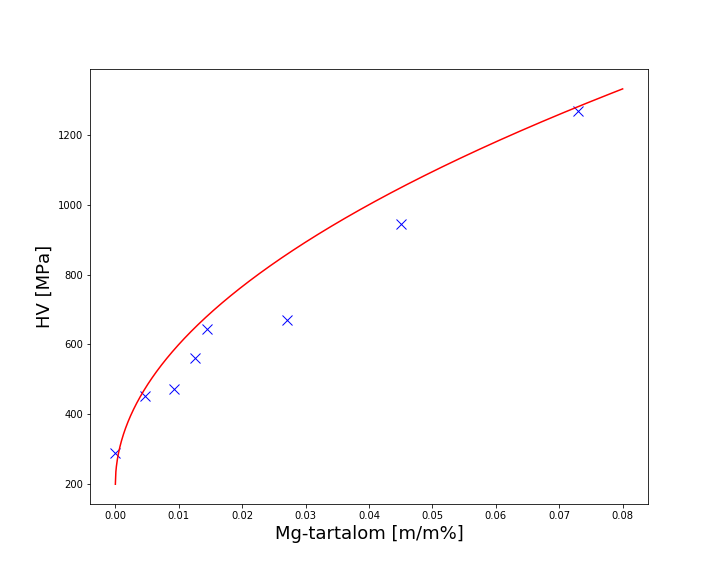
\includegraphics[width=0.75\textwidth]{./adatok/HV_illeszt.png}
\end{figure}

\par Ahol az illesztési paraméterek értékei a következők:

\begin{equation*}
 HV_0=(10273.02\pm2245.52)~MPa \quad \quad
 B = (337.92\pm35.82)~MPa \quad \quad
 m = 0.85\pm0.09
\end{equation*}

\par Ezután a különböző sebességeknél való benyomást vizsgálva, kivonva a mért erőt az illesztettből a fogazottság a következőképpen alakult:

\begin{figure}[H]
\centering
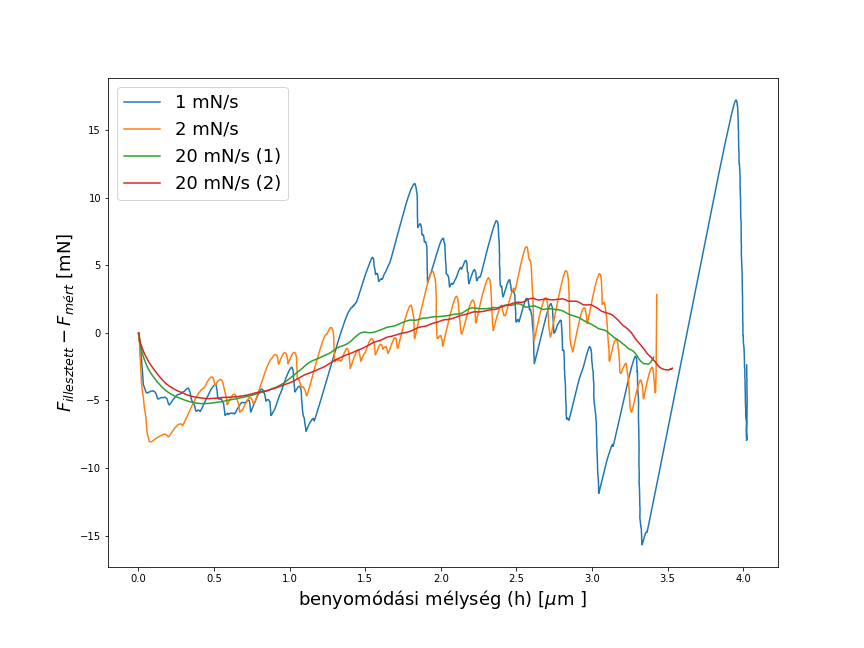
\includegraphics[width=0.75\textwidth]{./adatok/feladat3.png}
\end{figure}

\par Jól látható, hogy ahogy vártuk, a fogazottság legnagyobb mértékben kis sebességeknél jelenik meg. Az illesztett görbék ($f(h) = A\cdot h^{m}$) paraméterei a következők:

\begin{itemize}
\item 1 mN/s: $A = (29.52\pm0.13)~mN/(\mu m)^m$, $m = 1.311\pm0.004$
\item 2 mN/s: $A = (34.99\pm0.10)~mN/(\mu m)^m$, $m = 1.362\pm0.003$
\item 20 mN/s (1): $A = (31.64\pm0.21)~mN/(\mu m)^m$, $m = 1.457\pm0.006$
\item 20 mN/s (2): $A = (28.70\pm0.21)~mN/(\mu m)^m$, $m = 1.489\pm0.007$
\end{itemize}

\section{ Összegzés}

\par A kiértékelésünket többször ellenőrizve, arra a következtetésre jutottunk, hogy a $Cu, Ni$ minták valószínűleg nem tiszta anyagok, mert az irodalmi értéktől a keménységük nagyban eltért. 

\end{document}\grid
